\documentclass{beamer}
\usepackage{graphicx}
\usepackage{amsmath}
\usepackage{caption}

\usetheme{Madrid}

\title{Image Processing Workflow}
\author{Your Name}
\date{\today}

\begin{document}

% 标题页
\frame{\titlepage}

% 步骤 1:图像加载与灰度转换
\begin{frame}{1. Image Loading and Grayscale Conversion}
    \begin{block}{Step Explanation}
        The image is loaded using a Python imaging library and converted to grayscale. \\
        This reduces data complexity and focuses analysis on structural content.
    \end{block}

    \vspace{0.5cm}
    \begin{columns}
        \column{0.5\textwidth}
        \centering
        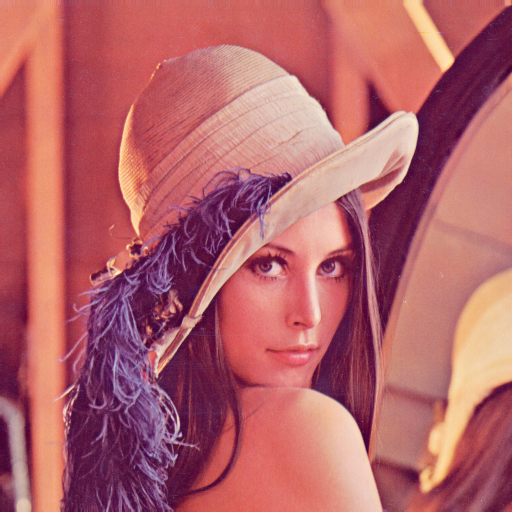
\includegraphics[width=\linewidth]{lena.jpg}
        \captionof{figure}{Original Color Image}

        \column{0.5\textwidth}
        \centering
        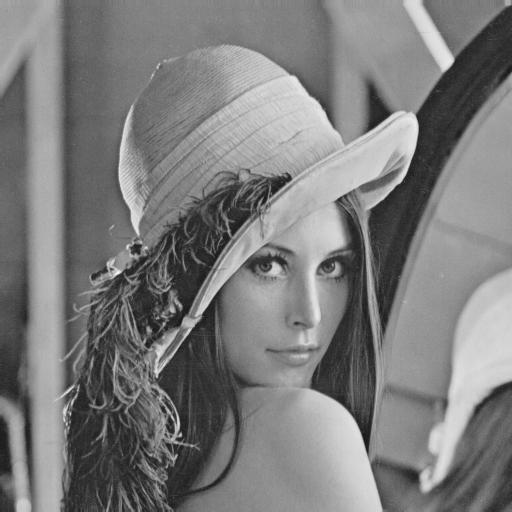
\includegraphics[width=\linewidth]{gray.jpg}
        \captionof{figure}{Grayscale Converted Image}
    \end{columns}
\end{frame}

% 步骤 2 和 3:缩放和居中裁剪
\begin{frame}{2. Rescaling and 3. Centered Cropping}
    \begin{block}{Rescaling with Aspect Ratio Preservation}
        The image is resized using high-fidelity interpolation to ensure one side reaches the target length ($2^N$), without distortion. \\
        The resized image is cropped to $2^N \times 2^N$, ensuring input uniformity without compromising important visual features.
    \end{block}

    \vspace{0.3cm}
    \begin{columns}
        \column{0.5\textwidth}
        \centering
        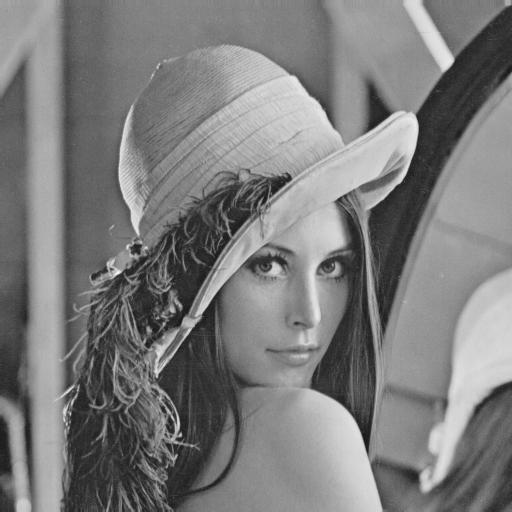
\includegraphics[width=\linewidth]{gray.jpg}
        \captionof{figure}{Before Rescaling}

        \column{0.5\textwidth}
        \centering
        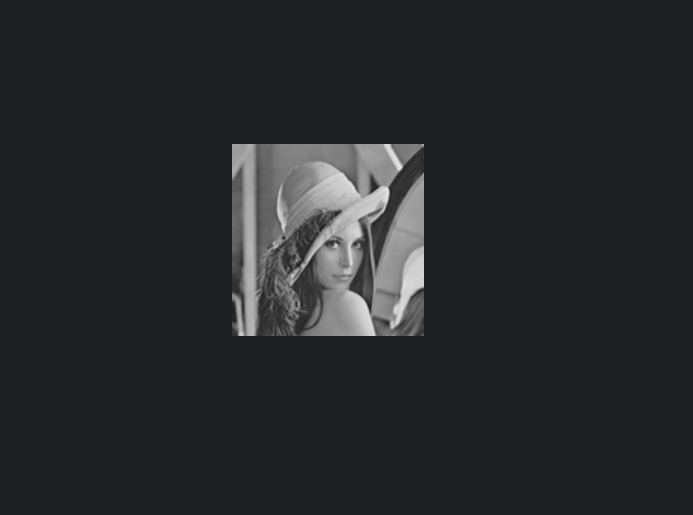
\includegraphics[width=\linewidth, height=5cm]{shuoxiao.png}
        \captionof{figure}{After Rescaling ($2^N$ Side)}
    \end{columns}
\end{frame}

% 步骤 4:矩阵输出
\begin{frame}{4. Matrix Output}
    \begin{block}{Step Explanation}
        The final image is converted into a matrix format suitable for: \\
        $\boldsymbol{\cdot}$ Mathematical operations (e.g., wavelet transforms) \\
        $\boldsymbol{\cdot}$ Storage and machine learning integration
    \end{block}

    \vspace{1cm}
    \centering
    \begin{tabular}{|c|c|c|}
        \hline
        128 & 135 & 142 \\
        \hline
        130 & 138 & 145 \\
        \hline
        125 & 132 & 139 \\
        \hline
    \end{tabular} \\
    \vspace{0.5cm}
    \small{Example of 3x3 image matrix (simplified)}
\end{frame}

% 步骤 5:从矩阵还原图像
\begin{frame}{5. Convert Matrix Information into an Image}
    \begin{block}{Concept}
        Each matrix element represents the gray value of a pixel. Using this matrix, we can reconstruct the grayscale image.
    \end{block}

    \vspace{0.3cm}
    \begin{columns}
        \column{0.5\textwidth}
        \centering
        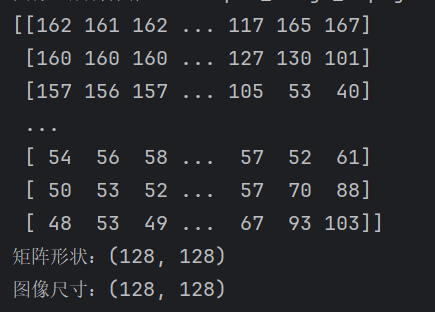
\includegraphics[width=\linewidth]{matrix_information.png}
        \captionof{figure}{Matrix Information}

        \column{0.5\textwidth}
        \centering
        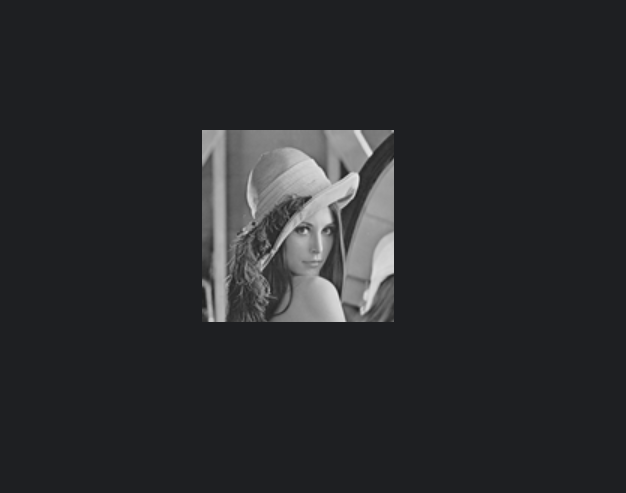
\includegraphics[width=\linewidth]{The_corresponding_image.png}
        \captionof{figure}{Reconstructed Image}
    \end{columns}
\end{frame}

\end{document}
